\documentclass[a4paper,12pt]{report}
\usepackage[utf8]{inputenc}
\usepackage[french]{babel}
\usepackage[T1]{fontenc}
\usepackage{graphicx}
\usepackage{subcaption}
\usepackage[colorlinks,urlcolor=blue,citecolor=red]{hyperref} %hyperlinks
\usepackage{xcolor} %color text
\usepackage[amsthm]{ntheorem} %theorems and co.
\usepackage{amsmath} %mathematical symbols
\usepackage{amssymb} %squares in itemize
\usepackage[page,toc,titletoc,title]{appendix} %appendices
\usepackage{natbib} %bibliography
\usepackage[nottoc,notlot,notlof]{tocbibind} %bind the table of contents to the bibligoraphy
\usepackage{packages/tikz-uml} %UML elements
\usepackage{silence} %silencing warnings
\WarningFilter{latex}{Text page}

%Defining custom commands for relational model
\newcommand{\attr}[1]{\emph{#1}}
\newcommand{\texit}[1]{\#\textsl{#1}}

%Redefining the appendices name to "Annexes" in toc and removing "Annexe" from appendice title
\renewcommand{\appendixtocname}{Annexes}
\appendixtitletocoff

%Redefining the appendices name to "Annexes" in the report
\renewcommand{\appendixpagename}{Annexes}

%Defining a new command for the horizontal lines
\newcommand{\HRule}{\rule{\linewidth}{0.5mm}}

%Defining custom environments
\theoremstyle{break}
\newtheorem*{userStory}{User Story}

\theoremstyle{break}
\newtheorem*{definition}{Définition}

\theoremstyle{break}
\newtheorem*{property}{Propriété}

\theoremstyle{break}
\newtheorem*{constraint}{Règle}

\theoremstyle{definition}
\newtheorem*{example}{Exemple}

\theoremstyle{remark}
\newtheorem*{remark}{\textbf{Remarque}}

\begin{document}
\pagenumbering{roman}
%----------------------------------------------------------------------------------------
%   TITLE PAGE
%----------------------------------------------------------------------------------------
\begin{titlepage}
\centering
%----------------------------------------------------------------------------------------
%   LOGOS SECTION
%----------------------------------------------------------------------------------------

\includegraphics[scale=0.5]{images/umLogo.png} %Université de Montpellier Logo
\hspace{\fill}

\includegraphics[scale=0.25]{images/fdsLogo.jpg} %Faculté de Sciences Logo
\hspace{\fill}

\includegraphics[scale=0.25]{images/lirmmLogo.png}~\\[2cm] %LIRMM Logo
%----------------------------------------------------------------------------------------
%   HEADING SECTIONS
%----------------------------------------------------------------------------------------
\textsc{\LARGE L3 CMI Informatique}\\[0.5cm]
\textsc{\Large \textbf{HLIN601} -- TERL3}\\[0.25cm]
\textsc{\Large \texttt{CourtCircuit}}\\[2cm]
%----------------------------------------------------------------------------------------
%   TITLE SECTION
%----------------------------------------------------------------------------------------
\HRule \\[0.4cm]
{\huge \bfseries RAPPORT \#$2$}\\[0.1cm]
\HRule \\[2cm]
%----------------------------------------------------------------------------------------
%   STUDENTS SECTION
%----------------------------------------------------------------------------------------
\begin{minipage}{0.5\textwidth}
\centering \large
\textbf{Bachar \textsc{Rima}}\\
\textbf{Othmane \textsc{Farajallah}}\\
\textbf{Wissem \textsc{Soussi}}
\end{minipage} \\[2cm]
%----------------------------------------------------------------------------------------
%   SUPERVISORS SECTION
%----------------------------------------------------------------------------------------
\begin{minipage}[b]{0.5\textwidth}
\begin{flushleft} \large
\emph{Responsable CMI Informatique :} \\
Anne-Elisabeth \textsc{Baert} \\
\end{flushleft}
\end{minipage}
~
\begin{minipage}[b]{0.4\textwidth}
\begin{flushright} \large
\emph{Encadrant :}\\
Eric \textsc{Bourreau}
\end{flushright}
\end{minipage}\\[1.5cm]
%----------------------------------------------------------------------------------------
%   DATE SECTION
%----------------------------------------------------------------------------------------
{\large \today}\\[1cm]
\hspace{\fill}
\vfill % Fill the rest of the page with whitespace
\end{titlepage}
%----------------------------------------------------------------------------------------
%   TABLE OF CONTENTS
%----------------------------------------------------------------------------------------
{
  \hypersetup{linkcolor=black}
  \tableofcontents
  \setcounter{page}{3}
}
%----------------------------------------------------------------------------------------
%   INTRODUCTION
%----------------------------------------------------------------------------------------
\chapter{Introduction}
\pagenumbering{arabic}
\setcounter{page}{1}
%----------------------------------------------------------------------------------------
%   CONTEXTE DU PROJET
%----------------------------------------------------------------------------------------
\section{Contexte du projet}
Dans ce rapport, nous nous consacrons à la description détaillée de la phase d'implémentation du projet intitulé \texttt{CourCircuit}\footnote{précédemment nommé \textbf{LaRuche}} à effectuer au sein du \textbf{LIRMM} (\textbf{L}aboratoire d'\textbf{I}nformatique, de \textbf{R}obotique et de \textbf{M}icroélectronique de \textbf{M}ontpellier) dans le cadre du module \textbf{HLIN601 -- TER} de la $3$\ieme{} année de licence en informatique \textbf{CMI} (\textbf{C}ursus \textbf{M}aster \textbf{I}ngénierie).

Le projet se déroule sous l'encadrement de Mme Anne-Elisabeth Baert, enseignante/chercheuse au sein du LIRMM dans l'équipe \textbf{MAORE} (\textbf{M}éthodes \textbf{A}lgorithmes pour l'\textbf{O}rdonnancement et les \textbf{Ré}seaux), en tant que responsable de la formation CMI informatique et M. Eric Bourreau, enseignant/chercheur au sein du LIRMM dans la même équipe \textbf{MAORE}, en tant que responsable pédagogique et encadrant du projet.

Le sujet du projet consiste en la création d'un site web représentant une interface de communication entre fournisseurs de produits locaux et leurs clients. Il est inspiré du site \og \href{https://laruchequiditoui.fr/fr}{La Ruche Qui Dit Oui} \fg traitant le même thème et répondant aux mêmes besoins, cependant adoptant une approche différente, surtout au niveau de la logistique et de l'architecture du site, afin de fournir une vision différente, voire plus optimisée de la gestion des interactions directes entre clients et fournisseurs.

Nous commencerons ce rapport en faisant un récapitulatif du contexte du projet, des problématiques traitées, et de la méthodologie et des outils de conception adoptés. De plus, nous proposerons une courte description des outils d'implémentation choisis pour la mise en \oe{}uvre. Après, nous procéderons à la description détaillée des outils d'implémentation et à la présentation des résultats obtenus. Enfin, nous conclurons en discutant les difficultés survenues lors du développement et les perspectives du projet.
%----------------------------------------------------------------------------------------
%   PRÉSENTATION DU LIRMM
%----------------------------------------------------------------------------------------
\section{Présentation du LIRMM}
\og Le [...] – LIRMM – est une unité mixte de recherche, dépendant conjointement de l'Université Montpellier et du Centre National de la Recherche Scientifique [(CNRS)]. Il est situé sur le Campus Saint-Priest de l'UM [(Figure \ref{fig:lirmmPhoto})].

\begin{figure}[!ht]
  \centering
  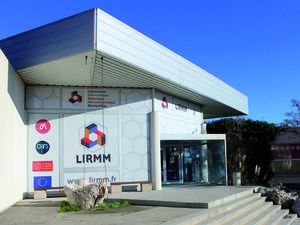
\includegraphics[scale=0.9]{images/lirmmPhoto.jpg}
  \caption{bâtiment 3 du LIRMM, Campus St. Priest}
  \label{fig:lirmmPhoto}
\end{figure}

Les travaux sont menés dans trois départements scientifiques de recherche, [(L’Informatique, La Robotique, et La Microélectronique)] eux-mêmes organisés en \og équipes-projet \fg.

Les recherches menées au LIRMM trouvent généralement une finalisation dans des domaines applicatifs aussi divers que la biologie, la chimie, les télécommunications, la santé, l'environnement... et dans les domaines propres du laboratoire : l'informatique, l'électronique et l'automatique.

Ses activités de recherche [le] positionnent [...] pleinement au coeur des sciences et technologies de l’information, de la communication et des systèmes. [En particulier,] les thématiques du département Informatique s’étendent des frontières des mathématiques à la recherche appliquée : algorithmique des graphes, bioinformatique, cryptographie, réseaux, bases de données et systèmes d'information [...], génie logiciel [...], intelligence artificielle [...], interaction homme-machine [...]. \fg{} \citep{lirmmPres}
%----------------------------------------------------------------------------------------
%   PROBLÈME, MÉTHODOLOGIE, OUTILS ET PLANNING
%----------------------------------------------------------------------------------------
\chapter{Problème, Méthodologie, et Outils}
%----------------------------------------------------------------------------------------
%   PROBLÈME
%----------------------------------------------------------------------------------------
\section{Problème}
Les consommateurs cherchent de \textit{plus en plus} à acheter des produits frais minimisant les étapes de \textit{processing}, alors que les producteurs cherchent à se libérer des centres d’achat et des intermédiaires de distribution.

Dans l’esprit du site francais \href{https://laruchequiditoui.fr/fr}{LaRucheQuiDitOui}, on souhaite implémenter une interface sous forme d'un \textbf{site web} d'\textit{e-commerce} permettant aux producteurs de vendre des sélections diversifiées de produits aux consommateurs en se regroupant dans des endroits précis de collecte.

Le site web offrira ainsi \textbf{tout ce dont il est nécessaire} aux consommateurs pour effectuer des commandes prépayées et précisera ensuite les points de collecte de produits les plus proches. D'autre part, il mettra à la disposition des fournisseurs la possibilité d'organiser ces points, de gérer la mise à jour des stocks et la mise en vente/prise de commandes par les clients, en se basant sur des algorithmes d'optimisation se portant aussi bien sur la gestion de la logistique, la préparation/facturation des commandes, que sur la redistribution/partage des produits entre les différents fournisseurs voisins.
%----------------------------------------------------------------------------------------
%   MÉTHODOLOGIE
%----------------------------------------------------------------------------------------
\section{Méthodologie}
Dans le but d'assurer une bonne gestion des ressources et d'offrir le plus de fonctionnalités possibles aux utilisateurs, en les implémentant itérativement dans des versions fonctionnelles et testées du site, nous avons opté pour une approche basée sur les \textbf{méthodes agiles} de développement, en particulier sur \textbf{XP}\footnote{\textit{eXtreme Programming}}.

En effet, la méthodologie de développement proposée par les méthodes agiles étant de plus en plus prépondérante en génie logiciel, nous avons décidé de l'utiliser pour la modélisation et l'implémentation de notre site web afin d'assurer le plus d'extensibilité et de flexibilité possibles.
%----------------------------------------------------------------------------------------
%   OUTILS DE CONCEPTION
%----------------------------------------------------------------------------------------
\section{Outils de conception}
Pour garantir une bonne modélisation du projet, en cohérence avec l'approche de la méthodologie discutée précédemment, nous avons explicité les spécifications fonctionnelles et organisationnelles de notre projet en se servant des outils suivants :
\begin{description}
  \item[\textit{user stories}]{des requis fournis par les utilisateurs décrivant en langage naturel les fonctionnalités qu'ils souhaitent avoir dans le site.}
  \item[diagrammes de cas d'usage]{des diagrammes dynamiques, souvent utilisés en \textbf{UML} pour décrire en haut niveau les fonctionnalités d'un système, en se servant de notions telles que \textbf{acteurs}, \textbf{cas d'usage}, \textbf{systèmes} et les \textbf{relations} entre chacune de ces entités.}
  \item[modèle EA]{un modèle \textbf{conceptuel} utilisé pour décrire les entités du projet ainsi que les associations décrivant leurs relations et comportements.}
  \item[schéma de base de données]{schéma en modèle \textbf{relationnel} composé des schémas des relations et des contraintes d'intégrité sur l'ensemble des relations, traduit généralement à partir du \textbf{modèle EA} et servant comme \textbf{modèle logique} lors de l'implémentation de la \textbf{base de données}.}
  \item[\textit{mockup storyboard}]{document de haut niveau offrant un moyen pour schématiser l'utilisation d'un projet, en positionant les différents éléments le composant, sans rentrer dans les détails de leur fonctionnement.}
\end{description}
%----------------------------------------------------------------------------------------
%   OUTILS D'IMPLÉMENTATION
%----------------------------------------------------------------------------------------
\section{Outils d'implémentation}
Afin de réaliser les impératifs de la partie conception du projet, nous avons prévu, pendant la partie de modélisation, d'utiliser principalement \textit{React.js}, \textit{JQuery}, \textit{Boostrap}, \textit{PHP} et \textit{MySQL}, ainsi que d'autres \textbf{API} pour l'implémentation de certaines parties du projet. Toutefois, après avoir compléter notre soutenance et suite à des recherches supplémentaires, nous avons décidé d'abandonner quelques technologies et de les remplacer par d'autres plus pertinentes afin d'obtenir un écosystème de travail plus cohérent et plus efficace.

Ce choix fût alimenté par plusieurs facteurs que nous discuterons plus en détail dans le chapitre \ref{chap:implementation_resultats} de ce rapport. Pour cette section, nous nous contentons simplement de fournir une courte description de l'ensemble de l'écosystème qui, en l'occurrence, est composé de :

\subsubsection{\textit{Front-end}}
\begin{description}
  \item [React.js :] une bibliothèque \textbf{JavaScript} créée par \textit{Facebook} et sortie en $2013$ pour la création des interfaces graphiques.
  \item [JSX :] (\textit{JavaScript XML}) une extension syntaxique du \textbf{JavaScript} permettant de simplifier la création des composants \textit{React} à travers une syntaxe à la \textbf{XML}.
  \item [Bootstrap :] un \textit{framework} \textbf{CSS} permettant la gestion du \textit{responsive web} du site.
\end{description}

\subsubsection{\textit{Back-end}}
\begin{description}
  \item [Node.js :] un environnement d'exécution \textbf{JavaScript} côté serveur gratuit et \textit{open-source} utilisant le moteur \textbf{JavaScript V8} de \textit{Google Chrome}.
  \item [Express :] un framework gratuit et open-source pour construire des applications web et des \textbf{API}s sur \textbf{Node.js}.
  \item [MariaDB :] un serveur de base de données gratuit et open-source remplaçant \textbf{MySQL} tout en restant compatible avec ce dernier.
\end{description}

\subsubsection{Editeur de texte}
\noindent
Pour la rédaction du code de notre projet, nous avons choisi unanimement d'utiliser l'éditeur de texte gratuit, open-source et multiplateforme \textbf{Atom} pour son architecture basée sur \textbf{Node.js}. En effet, cette architecture permet de personnaliser son utilisation et de le rendre plus souple via des modules téléchargeables par le biais de son gestionnaire de packages \textbf{APM} (\textit{Atom Package Manager}).

\begin{figure}[!ht]
  \centering
  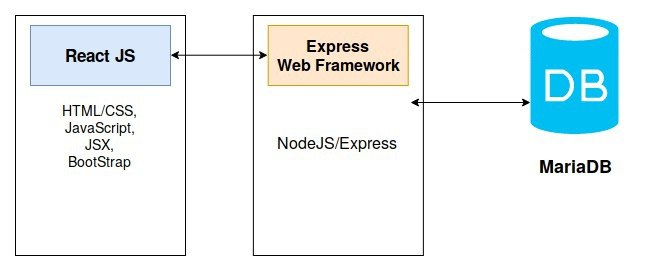
\includegraphics[scale=0.5]{images/website_architecture.jpeg}
  \caption{L'architecture des technologies utilisées en CourtCircuit}
  \label{fig:website_architecture}
\end{figure}

Par conséquent, l'architecture des technologies choisies pour l'implémentation de notre projet est illustrée dans la figure \ref{fig:website_architecture}.
%----------------------------------------------------------------------------------------
%   IMPLÉMENTATION
%----------------------------------------------------------------------------------------
\chapter{Implémentation et Résultats}
\label{chap:implementation_resultats}
%----------------------------------------------------------------------------------------
%   APPLICATION WEB MONOPAGE
%----------------------------------------------------------------------------------------
\section{Application web monopage}
Une application web est dite monopage quand elle est concu pour ne pas avoir plusieurs fichiers
HTML relatives aux differentes pages du site, mais plutot une unique page HTML avec les rélatives ressources
Javascript et CSS permettant d'afficher les differentes pages dinamiquement.
Avec un site web classique le navigateur affiche simplement les pages envoyées par le serveur et lui transmet les actions de l’utilisateur.
Le navigateur prend donc un rôle plus important que dans un site web classique, puisqu'il ce charge de toute la logique applicative,
en reagissant aux actions de l'utilisateur. Le serveur devient donc responsable que des ressource a fournir en effectuant de son coté
que les verifications de securité necessaire avant qu'il n'envoie quelque ce soit.
C'est pour cela que la page web unique deviens une veritable application, qui tourne coté client pour fluidifier l'experience de l'utilisateur:
en evite de charger a chaque requette de l'utilisateur une page entiere, et on change la page en fonction du serveur partiellement.

%----------------------------------------------------------------------------------------
%   FRONT-END
%----------------------------------------------------------------------------------------
\section{Front-end }
%----------------------------------------------------------------------------------------
%   REACT-JS
%----------------------------------------------------------------------------------------
\subsection{React.js}
%----------------------------------------------------------------------------------------
%   BOOTSTRAP
%----------------------------------------------------------------------------------------
\subsection{Bootstrap et Font-Awesome}
\textbf{Bootstrap} est un framework pour le developpement front-end, donc coté client d'un site web.
Il est pricipalement un framework CSS mais embarque aussi des composants Javascript et HTML.
En utilisant un systeme de grille pour gerer le Layout d'une page Bootstrap est capable de changer dynamiquement
ce Layout par rapport à la taille de la fenetre du navigateur permettant d'avoir un site responsive utilisable
avec praticité soit sur les petits ecrans tel que smartphone ou tablet, comme sur les grands comme un moniteur ou un téléviseur.
Grace à l'ensemble de classes css, Bootstrap permet un developpement du site-web rapide tout en permettant de personnaliser le design
en ajoutant peut de lignes de code. On a par exemple des boutons, des formulaires, des navbars,
des accordilons, des carousels, tous esthetiques et personalisables avec l'ajout d'animations javascript qui est de base fait avec
JQuery.
\begin{figure}[!ht]
  \centering
  
\includegraphics[scale=0.4]{images/bootstrap.png}
  \caption{Navbar du site fait avec Bootstrap}
\end{figure}
Sur notre site on a donc utilisé Bootstrap pour tout ce qu'on a mentionné, en evitant de reinventer la roue et definir
l'eshtetique de chaque element HTML à partir de zerò.
\textbf{Font-awesome} a été crée pour etre utilisé avec Bootstrap et c'est un outils qui permets d'utiliser les icons comme des polices d'écritures
qui peuvent subir des changement de style avec CSS, SASS ou LESS.
Avec ces deux frameworks, chaque composante REACT a été esthétiquement personnalisée, nottament:
\begin{itemize}
  \item L'entete du site, qui est un Navbar (barre de navigation) responsive et "collapsable" pour les écran de petite taille;
  \item Le footer du site, en utilisant des icones Font-awesome pour les liens vers d'autres pages.
\end{itemize}
%----------------------------------------------------------------------------------------
%   CHARTE GRAPHIQUE
%----------------------------------------------------------------------------------------
\subsection{Charte graphique}
Pour le site web, etant principalement un site de commerce de fruits et legumes, nous avons pensé d'utiliser des couleurs comme le vert et
l'orange, qui donnent aux images des produits à vendre une embience de nature et de fraicheur. De plus les fonts, couleurs et logos sont sombres et simples.
\newpage
\begin{figure}[!ht]
  \centering
  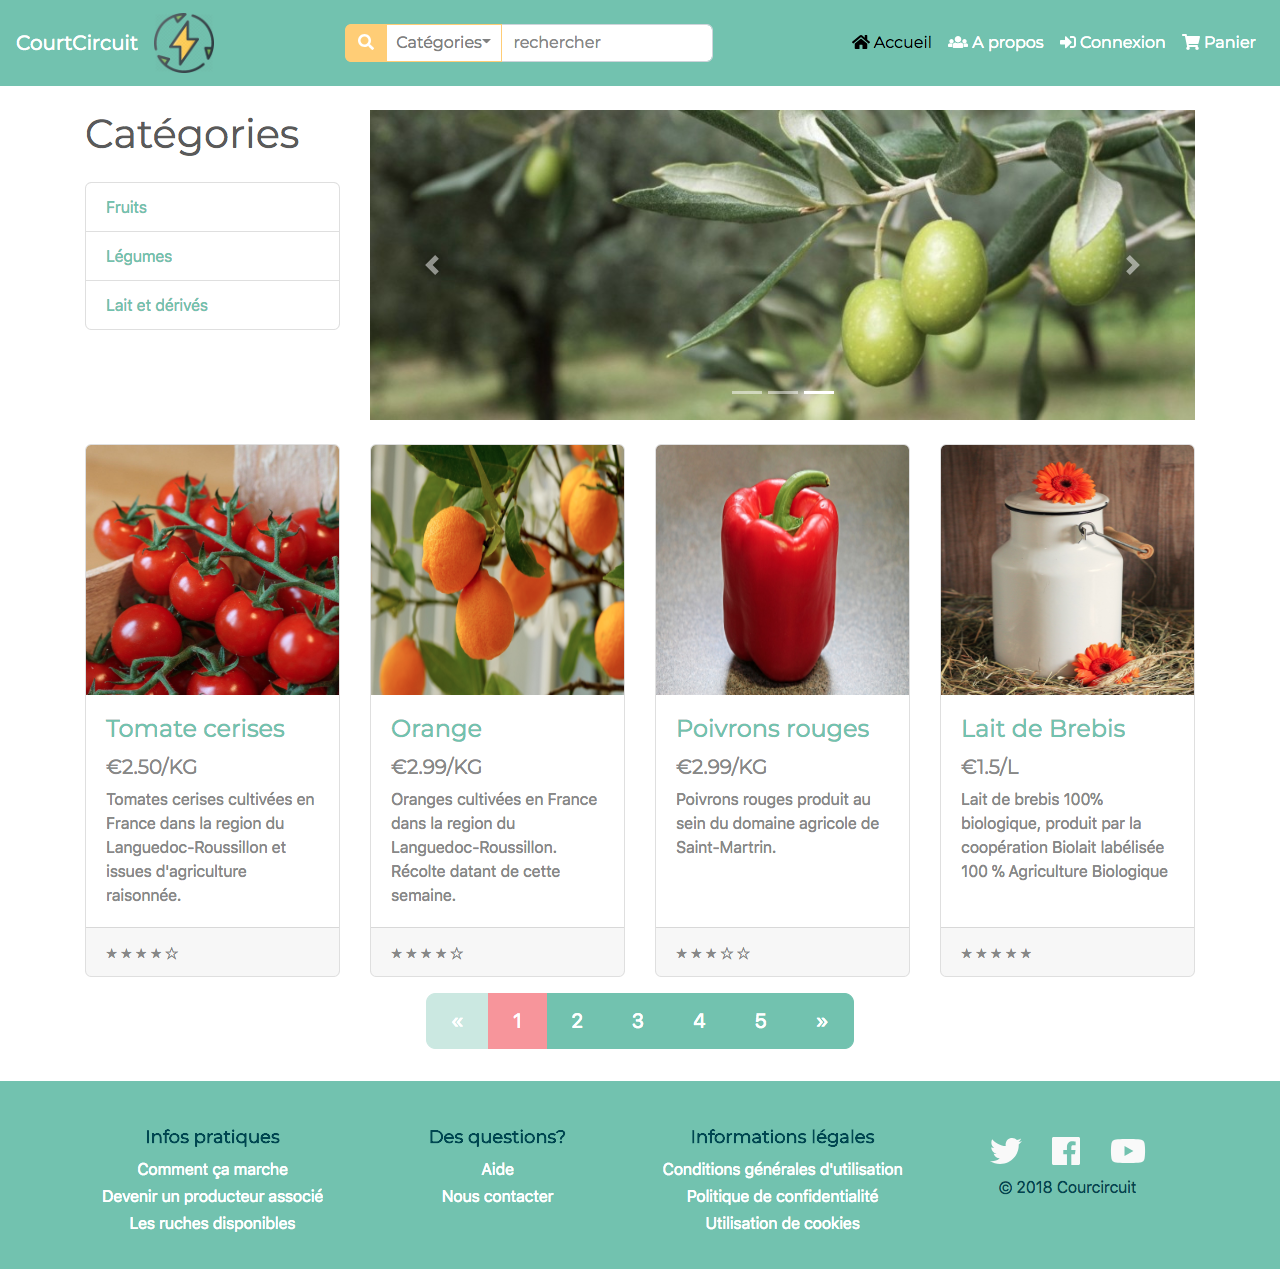
\includegraphics[scale=0.3]{images/accueil.png}
  \caption{Page d'accueil du site web}
\end{figure}
%----------------------------------------------------------------------------------------
%   BACK-END
%----------------------------------------------------------------------------------------
\section{Back-end}
Pour la partie back-end, nous avons décidé d'utiliser \textbf{Node.js}/\textbf{Express.js} pour le serveur et \textbf{MariaDB} pour la base de données. Nous détaillerons les raisons et les résultats d'utilisation
%----------------------------------------------------------------------------------------
%   NODE.JS
%----------------------------------------------------------------------------------------
\subsection{Node.js}
\begin{figure}[!ht]
  \centering
  
\includegraphics[scale=0.04]{images/nodejs_icon.png}
  \caption{le logo de \textbf{Node.js}}
\end{figure}

\textbf{Node.js} est un environnement d'exécution \textbf{JavaScript} côté serveur utilisant le moteur \textbf{JavaScript V8} de \textit{Google Chrome}. Il est libre, gratuit et doté d'une efficacité et d'une légèreté provenant de sa modélisation événementielle, monothread et non-bloquante et de son architecture modulaire. Sa facilité d'usage et son extensibilité est dûe aussi à son gestionnaire de paquets \textbf{NPM} (\textit{Node Package Manager}) considéré comme l'un des plus larges écosystèmes de librairies open-source au monde.

\textbf{Node.js} est une technologie récente qui est de plus en plus utilisée, surtout en développement web avec les architectures \textbf{MERN} (\textit{MongoDB Express React Node}) et \textbf{MEAN} (\textit{MongoDB Express Angular Node}). Par suite, ceci nous a motivé à l'intégrer dans notre projet au vu de ses nombreuses avantages.

En premier, notre choix de \textbf{Node.js} découle du fait qu'il permet d'écrire du code \textbf{JavaScript} du côté serveur. Cette particularité nous a permis d'unifier la rédaction du code en un seul langage, pour les côtés client et serveur. En effet, l'unification du code a rendu possible à l'ensemble du groupe de participer au débogage du projet entier sans aucune restriction liée à la maîtrise d'un langage ou l'autre.

Outre l'unification du code, étant donné que nous aurons besoin de gérer un ensemble important de données dans le cadre de notre projet, l'aspect monothread et non-bloquant de \textbf{Node.js} assure une performance fluide que nous ne trouverons pas forcément avec d'autres technologies back-end, utilisant généralement des modèles multi-processus ou multithread.

Enfin, \textbf{Node.js} est le choix par défaut pour une architecture utilisant \textbf{React.js}\footnote{bien que pas le seul}, ce qui nous a encouragé davantage à s'en servir.

Dans le cadre de notre projet, nous avons principalement utilisé \textbf{Node.js} pour la création d'une \textbf{API} côté serveur permettant d'interfacer avec la base de données. Ceci fût concrétisé par la création des objets pour les différentes entités manipulés (\textit{Client, Utilisateur, Produit, $\dots$}), en s'appuyant sur des concepts de la programmation orienté-objet. Par conséquent, nous avons pu factoriser le code pour éviter les redondances et  améliorer sa lisibilité lors de l'exécution des requêtes sur la base de données.

D'autre part, nous nous sommes également servi de \textbf{Node.js} pour l'utilisation du framework \textbf{Express} que nous détaillerons dans la section suivante.
%----------------------------------------------------------------------------------------
%   EXPRESS
%----------------------------------------------------------------------------------------
\subsection{Express}
\begin{figure}[!ht]
  \centering
  
\includegraphics[scale=0.4]{images/express_icon.png}
  \caption{Le logo de \textbf{Express}}
\end{figure}

\textbf{Express} est un framework minimaliste gratuit et open-source, devenu standard pour construire des applications web et des \textbf{API}s côte serveur sur \textbf{Node.js}. Il s'appuie sur des concepts \textbf{MVC} (\textit{Model View Controller}) et offre plusieurs services notamment l'utilisation de moteurs de templates (\textit{EJS (Embedded JavaScript), Handlebars, et Jade}), l'utilisation de \textit{middleware}, la gestion des routes et des formulaires, $\dots$.

Dans le cadre de notre projet nous nous sommes principalement servi d'\textbf{Express} pour la gestion côté serveur des routes implémentées par \textbf{React} en implémentant les opérations \textbf{CRUD} (\textit{Create, Read, Update, Delete}) correspondantes.
%----------------------------------------------------------------------------------------
%   MARIADB
%----------------------------------------------------------------------------------------
\subsection{MariaBD}
\begin{figure}[!ht]
  \centering
  
\includegraphics[scale=0.4]{images/mariadb_icon.png}
  \caption{Le logo de \textbf{MariaDB}}
\end{figure}

En général, le serveur de base de données \textbf{MongoDB} est le choix par défaut pour une architecture incluant \textbf{React}, \textbf{Node.js} et \textbf{Express}. Ceci est dû principalement à sa modélisation \textbf{NoSQL} basée sur des documents au format \textbf{JSON} facilitant la récupération et le stockage des données à travers une technologie back-end utilisant \textbf{JavaScript} telle que \textbf{Node.js}.

Toutefois, vu que nous avions déjà traduit notre \textbf{modèle EA} (cf. Figure \ref{fig:modele_EA}) en \textbf{modèle relationnel}, et vu que le serveur de la faculté qui nous a été attribué pour le déploiement de notre site n'hébérgeait pas un serveur \textbf{MongoDB} mais hébérgeait bien son contrepartie \textbf{MySQL}, nous avons opté pour un \textbf{SGBD} relationnel classique, notamment \textbf{MariaDB}.

\textbf{MariaDB} est un serveur de base de données gratuit et open-source, assurant l'interopérabilité avec \textbf{MySQL}, qui fût introduit par les créateurs de \textbf{MySQL} suite à l'achat de ce dernier par \textbf{Oracle}. Il s'agit en réalité d'un fork communautaire de \textbf{MySQL} qui est mis à jour plus souvent que \textbf{MySQL}.

Pour toutes ces raisons, nous avons ainsi décidé d'adopter \textbf{MariaDB} comme \textbf{SGBD} de notre base de données.

Pour interfacer \textbf{Node.js} et \textbf{MariaDB} nous avons eu recours au \textit{package} \og \texttt{mysql} \fg que nous avions téléchargé via \texttt{npm}. Le package contient l'ensemble des fonctionnalités permettant de se connecter à la base de données et d'exécuter des requêtes \textbf{SQL} là-dessus.

\begin{figure}[!ht]
  \centering
  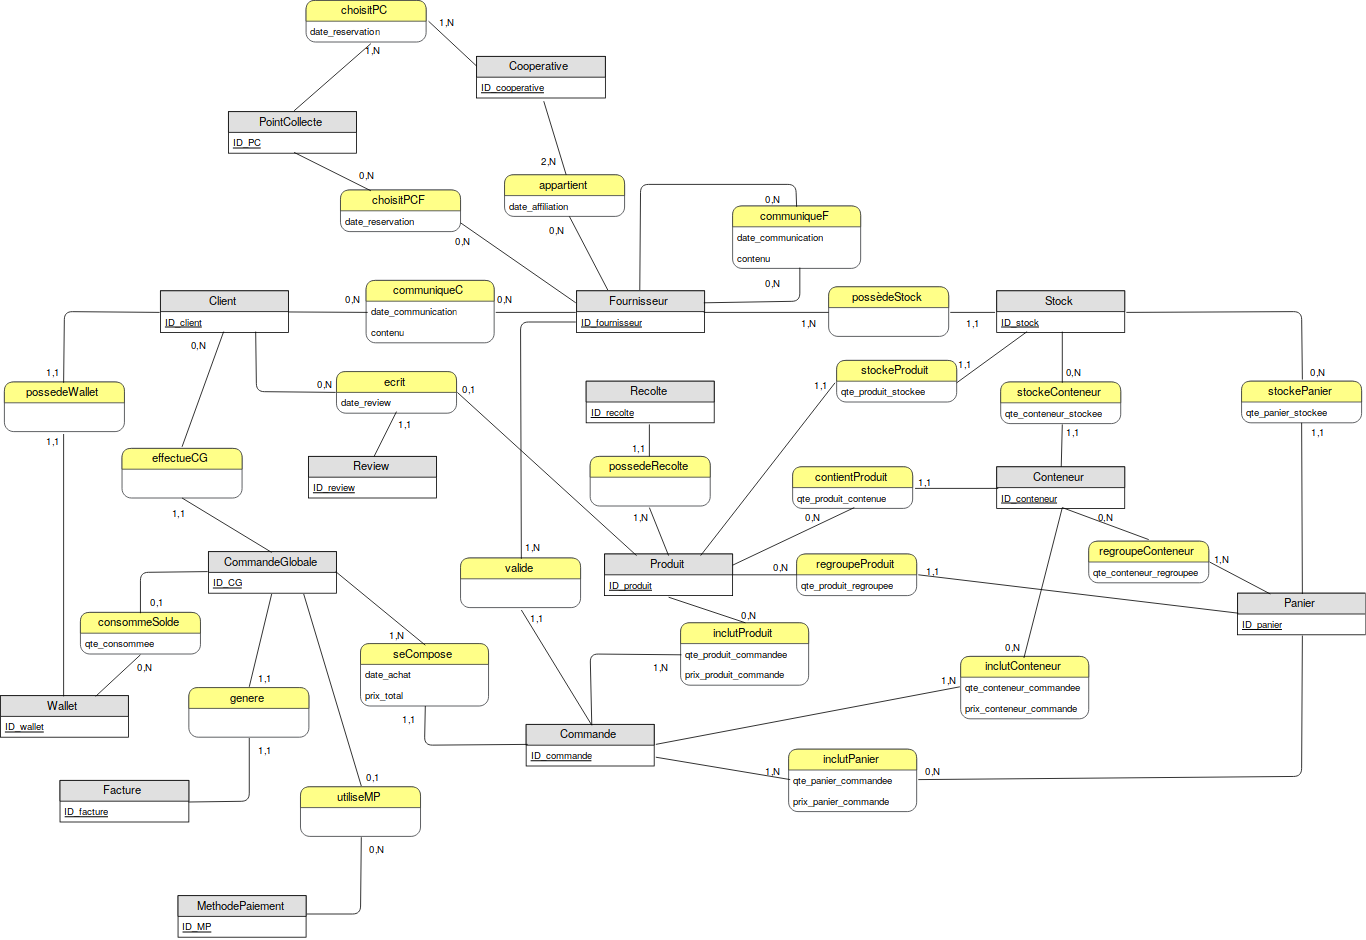
\includegraphics[scale=0.35]{images/er_model.png}
  \caption{Modèle Entité-Association}
  \label{fig:modele_EA}
\end{figure}

\newpage
%----------------------------------------------------------------------------------------
%   RESULTATS
%----------------------------------------------------------------------------------------
\section{Résultats}
%----------------------------------------------------------------------------------------
%   CONCLUSION
%----------------------------------------------------------------------------------------
\chapter{Conclusion}
%----------------------------------------------------------------------------------------
%   DIFFICULTÉS SURVENUES
%----------------------------------------------------------------------------------------
\section{Difficultés survenues}
On a rencontré des nombreux difficultés pendant le développement du projet, notamment sur la maîtrise de
nouveaux outils jamais utilisés auparavant: React, JSX, Express etc..
On a eu le sentiment d'avoir passé trop de temps dans la partie de la modélisation et conception en se retrouvant
avec 3 mois (qui ne sont pas entièrement dédiés non plus) pour la réalisation du site.
De plus, on a vu des concepts théoriques nouveaux comme le design pattern MVC, le concept d'une application web monopage,
et tous les outils conventionnellement utilisés pour des projets javascript : Babel, Npm, Node, React, Jsx etc ...
La compréhension et la pris en main de ces outils ont eu une partie importante du projet avant de commencer à les utiliser dans la pratique.
Une autre limitation a été le serveur d'hébergement du département informatique, qui a mis en place des environnements node et npm non mis a jours,
et qui nous n’a pas cree une base de données  dediee a notre projet comme c’etait prevu sur le site SIF. En manque des permissions necessaires, nous n’avons pas reussi a le faire nous-meme non plus, bien que nous avions signale ceci au parties concernees.


%----------------------------------------------------------------------------------------
%   PERSPECTIVES
%----------------------------------------------------------------------------------------
\section{Perspectives}
\label{sec:perspectives}
Outre les fonctionnalités que nous avons jugées essentielles au projet, nous avons pensé à ajouter
des fonctionnalités supplémentaires une fois celles de base établies. En effet, plusieurs extensions
sont possibles afin de proposer aux utilisateurs un choix plus diversifié et plus complet.
Dans ce cadre, nous avons prévu de donner aux clients la possibilité de régler des achats à l'aide
d'une carte bancaire mais également à l'aide de services de paiements en ligne tels que Paypal.
En addition, nous pourrions également internationaliser le site et son concept en proposant des versions
en plusieurs.
Le projet nous interesse et nous avons envie de le continuer comme projet personnel au delà du parcours d'études.
%----------------------------------------------------------------------------------------
%   APPORT PERSONNEL
%----------------------------------------------------------------------------------------
\section{Apports personnels}
Tout au long du projet, chaque difficulté rencontrée, qu'était une nouvelle expérience enrichissante. L'apprentissage de nouveaux concepts de programmation et de gestion de projet et la maîtrise de nouvelles technologies web, que nous n'avions guère manipulé au préalable, était un défi profondément apprécié. En particulier, nous avons eu la chance de profiter des richesses offertes par JavaScript dans différents contextes, ce qui a radicalement changé notre perception du langage.

Nous sommes convaincus que, jusqu'à présent, ce projet fût le plus intéressant, quoique le plus exigeant, parmi les projets auxquels nous avions participé. De plus, nous sommes bien ravis par les connaissances acquises qui prouverons certainement utiles ultérieurement dans nos formations futures mais également dans nos démarches professionnelles.
%----------------------------------------------------------------------------------------
%   ANNEXES
%----------------------------------------------------------------------------------------
\begin{appendices}
\end{appendices}
%----------------------------------------------------------------------------------------
%   BIBLIOGRAPHIE
%----------------------------------------------------------------------------------------
\bibliographystyle{agsm}
\bibliography{mybib}
\end{document}
